%%==============
%%==============
\section{Optimization study}

This section describes the changes that have to be included in \texttt{main} and \texttt{data} files for running optimization studies. An additional parameter file is required in this case:

\begin{itemize}
 \item opt.prm (or opt.xml): This file is used ONLY if in the main file section \texttt{Simulator}, subsection \texttt{Analysis type} is set to \texttt{Optimization}. The file is used to specify the required information to run an optimization simulation. Two optimization examples for cathode electrode are shown in the example folder.
\end{itemize}

In case that the user wants to run an optimization study using the GUI, the file opt.xml should be also loaded.


%-----
\subsection{Graphical user interface}
A project for an optimization study using the OpenFCST GUI is made of three files:

\begin{itemize}
 \item \texttt{main.xml} contains the main selections for OpenFCST, such as the type of application, nonlinear solver, and type of study to be performed, i.e. one analysis run or a parametric analysis run.
 \item \texttt{data.xml} contains the parameters to setup the simulation for the selected application.
 \item \texttt{opt.xml} is an optional file used to setup parameters for optimization.
\end{itemize}

The following steps should be followed in case the user is creating a new project or opening a new one:

\begin{enumerate}
 \item Starting a new project: After the data file has been generated, an optimization file may be also generated, depending on if you have compiled OpenFCST with Dakota.
 \item Opening an Existing Project: After specifying the location of the data file, you may load the optimization parameter file. 
\end{enumerate}

In case the user wants to edit the GUI's \textbf{settings.ini} file, the following parameter can be also modified:

\begin{itemize}
 \item \textcolor{grey}{\textbf{optFileName:}} The name of the optimization file which OpenFCST will create when generating a new Project.
\end{itemize}


%-----
\subsection{The \texttt{main} file}
In the \texttt{Simulator} section of the \texttt{main} file, the parameter \texttt{Analysis type} should be set to \texttt{Optimization} when an optimization study is to be performed. The file that includes all optimization parameters should be included in subsection \texttt{Optimization}. There are only two entries in this subsection:
\begin{itemize}
 \item \texttt{optimization parameter file name}: Enter here the name of the optimization file. By default, if using the GUI, opt.xml should be used.
 \item \texttt{Dakota direct}: Set to true if you would like OpenFCST to directly interact with Dakota, i.e. OpenFCST will call Dakota as needed to run the optimization simulation. If set to false, then OpenFCST will run once and output a file that Dakota can read. In this case Dakota would be the optimization driver.
\end{itemize}


% 
% 
% \subsection{Parameter/Optimization Application File}
% 
% 
% \item
% \texttt{opt\_app\_parametric\_default.prm}
% 
% The \texttt{opt\_app\_parametric\_default.prm} is used when carrying out parametric studies.
% 
% 
% 
% \begin{lstlisting}
% ######################################################################
% #
% #  This file is used to run a multi-dimensional parametric study. 
% #  See end of file for list of possible design variables.
% #
% ######################################################################
% 
% subsection Optimization Parameters
%   
% #### NOTE THAT THIS SECTION ONLY EXISTS WHEN RUNNING IN OPTIMIZATION MODE ###
% ####----------------------------------------------------------------------###
%     subsection Optimization Program Options
%       set Use dakota input file = false                               # (default) false
%       set Dakota_Input_File = dakota_input.in                 # not needed if -Use dakota input file = false- 
% 
%       set Optimization method = multidim_parameter_study      # multidim_parameter_study | optpp_q_newton | nl2sol | ncsu_direct
%     end
% 
%     subsection Design Variables
%       set num_design_variables = 1                    # 2
%       set DV_0_name = V_cell                                          # P_cell 
%       set DV_1_name = T_cell                                          # P_c   | RH_a
%       set DV_2_name = prc_Pt_c                                        # RH_c  | prc_Pt_c
% 
%       #######   Lower Bound                    #######
%       ####### lb < -1e30 for -inf #######
%       #---------------------------------#
%       set DV_0_lb = -1.1                      # V # Changed to -1.1, force dekota to start at -1.1
%       set DV_1_lb = 303                               # K #  
%       set DV_2_lb = 0.2                               # % # 
% 
%       #######  Upper Bound                    #######
%       ####### ub > 1e30 for inf #######
%       #-------------------------------#
%       set DV_0_ub = -0.1                      # V # 
%       set DV_1_ub = 353                               # K # 
%       set DV_2_ub = 0.5                               # % #
% 
%       #######                                                 Parameter Study Partitions                                                #######
%       ### NOTE: Evaluated at n+1 points between lower and upper bound ###
%       ###-------------------------------------------------------------###
%       set DV_0_partition = 50
%       set DV_1_partition = 8
%       set DV_2_partition = 10
%       end
% 
%       subsection Responses
%         set num_objectives = 1
%         set num_nl_constraints = 0                    # (default) 0
%         set num_eq_constraints = 0                    # (default) 0
% 
%         set RESP_0_name = current
%       end
%   end
% \end{lstlisting}
% 
% 
% 
% 
% Located at the bottom of all \texttt{opt\_app} files in both parametric \& optimization is a list of design variables available for the user to carry out a parametric studies or optimization. As of \textbf{1-SEP-2013} the following table lists the current parameters that can be passed to DAKOTA for parametric studies/ optimization.
% 
% If the user requires additional variables for parametric/optimization studies, modification of the \\ \texttt{dakota\_application.cc} file should be carried out. 
% 
% \bigskip
% 
% \begin{lstlisting}
%       ######### List of Possible Design Variable Names #########
%       #########----------------------------------------#########
% #     //              Conventional_CL.cc
% #     V_Pt_c | V_Pt_a         // Platinum loading per unit volume [mg/cm3]    (Cathode | Anode)
% #     prc_Pt_c | prc_Pt_a                     // Platinum loading on support [%wt]            (Cathode | Anode)
% #     prc_N_c | prc_N_a                               // Electrolyte loading [%wt]                    (Cathode | Anode)
% #     Av_c | Av_a                                                     // Active area [cm^2/cm^3]                      (Cathode | Anode)
% 
% #     //              Agglomerate_CL.cc
% #     r_agg_c | r_agg_a                       // Radius of the agglomerate [nm]               (Cathode | Anode)
% #     r_agg                                                           // Radius of the agglomerate [nm] **possibly redundant**
% #     epsilon_agg_c | epsilon_agg_a           // Agglomerate porosity                         (Cathode | Anode)
% #     epsilon_agg                                                                     // Agglomerate porosity **possibly redundant**
% 
% #     //              Operating_Conditions.cc
% #     V_cell                                  // Cell Voltage
% #     T_cell                                  // Cell Temperature  
% #     dV_a                                            // Voltage drop in the Anode
% #     P_c | P_a                               // Pressure                                     (Cathode | Anode)
% #     
% #     RH_c | RH_a                             // Relative Humidity                            (Cathode | Anode) 
% #     OCV                                                             // Open Circuit Voltage
% 
% #     //              Geometries.cc 
% #     L_CCL | L_ACL                                   // CL thickness                                 (Cathode | Anode)
% #     L_CGDL | L_AGDL                         // GDL thickness                                (Cathode | Anode)
% #     L_CMPL | L_AMPL                         // MPL thickness                                (Cathode | Anode) 
% #     Ch_width                                                        // Channel Width                                (Cathode | Anode)
% 
% \end{lstlisting}
% 
% 
% 
% \paragraph{Optimization Program Options:}
% 
% The \texttt{Optimization Program Options} of the \texttt{opt\_app} parametric file is responsible for telling OpenFCST whether it is required to formulate its own \texttt{dakota\_input.in} file or if you are supplying DAKOTA with a predefined input file (\textit{line 13 \& 14}). 
% 
% 
% \paragraph{``Use dakota input file'' \& ``Dakota\_Input\_File'':}
% 
% If \texttt{Use dakota input file} is set to \texttt{false} then OpenFCST will pass on the information specified in the \texttt{opt\_app\_parametric\_default.prm} file and DAKOTA will print out a new \texttt{dakota\_input.in} at run time. If however it is set to \texttt{true} we are telling OpenFCST that we have already specified an input file and that DAKOTA should use this directly rather than reading the information from the rest of the \texttt{opt\_app} file.
% 
% \paragraph{Note:} 
% 
% For completeness \texttt{``Use dakota input file'' \& ``Dakota\_Input\_File''} have been included in the default parametric file, however, when the user is not using their own \texttt{dakota\_input.in} file both line 13 \& 14 can be deleted.
% 
% Given that in most cases the user specifies all the parametric \& optimization information in the \texttt{opt\_app} file. The following descriptions will be relevant for cases when \texttt{Use dakota input file = false}.
% 
% \paragraph{Optimization Method:}
% 
% The \texttt{Optimization method} command is used to specify the type of study that is being carried out (optimization, parametric study, least squares fit, ...) for additional information on \texttt{Optimization methods} see section \ref{Optimization_using_FCST}. In our case we are looking to carry out a parametric study so the \texttt{multidim\_parameter\_study} should be specified.
% 
% \paragraph{Design Variables:}
% In the design variables section (\textit{line 19-45}) we specify the number of design variables that we want to change (\textit{line 20}), the upper and lower bounds for that variable (\textit{line 25-37}), and the number of points that we want to evaluate between the upper and lower bounds (\textit{line 39-45}).
% 
% 
% \paragraph{num\_design\_variables:}
% In the example above we have specified one design variable \texttt{V\_cell} for a  single parametric study. The corresponding upper, lower bounds, and partitions can be found at line 28, 35, and 42.
% 
% If the user wants to conduct a multi-dimensional parametric study we would simply change \texttt{num\_design\_variables} value from one to whatever number of variables required. In the example about we have the capabilities of increasing the number of variables to three. If the user requires more variables than this the user can simply add additional \texttt{DV\_\#\_name} and the corresponding upper, lower bound and partitions. 
% 
% \paragraph{Note:} The upper and lower bound of the voltage have been set to negative. This is because DAKOTA will vary its parameters from the lowest value to the highest value (In the non-negative case this is from 0.1 - 1.1 [V]). 
% 
% During the solving process OpenFCST uses the last mesh data and node values as the initial starting point for the next point  evaluation. As the function evaluations become more difficult as we enter the mass transport region (\texttt{V\_cell of 0.3 - 0.1}) the time taken to evaluate these points is much longer. If we change the voltage values to their negative the parametric study will go from 1.1 to 0.1 [V], this in turn decreases the solving time and allows the solver to use the previous values as appose to starting at the 0.1 [V] (the most difficult case). 
% 
% Additional advantages as well as reduced time is that in some cases if the solver begins at lower voltages (e.g. 0.1 [V]) the solver is unable to to converge due to the low oxygen values however if the solver starts at the 'easier case' (high voltages 1.1 - 0.8 [V]) it will carry on the previous solutions and be able to converge at the lower voltages.
% 
% 
% 
% \paragraph{Responses:}
% The response section of the \texttt{opt\_app} parametric file, specifies the number of outputs desired in the \texttt{dakota\_tabular.dat} data file, in our case there is \textsc{only one} objective value (\textit{Current Density [$A/cm^2$]}) line 52.
% 
%  It also is responsibly for specifying the type and number of constraints. There are two types of constraints; Equality (\textit{line 49}) and Inequality (\textit{line 50}), in general we do not typically use constraints in parametric studies so this section will be covered in more detail in the \textbf{optimization section}.
% 
% 
% 
% % Closing file numbering (3 main files)
% %-----------------------
% \end{enumerate}
% 
% 






%-----------------------------------------------------------------------------------------------------
%---------------------                  Running OpenFCST
%---------------------                  Optimization
%-----------------------------------------------------------------------------------------------------
% 
% 
% \section{Optimization using OpenFCST} \label{Optimization_using_FCST}
% When running an Optimization study the user requires three files, as seen above with parametric studies. The only difference however is that we change out(\textit{alter})  the third file to an optimization file/format.
% 
%  \texttt{opt\_app\_optimization\_default.prm}
% 
% \begin{lstlisting}
% ######################################################################
% #
% #  This file is used to run the optimization interface.  
% #  See end of file for a list of optimization variables.
% #
% ######################################################################
% 
% subsection Optimization Parameters
% 
% #### NOTE THAT THIS SECTION ONLY EXISTS WHEN RUNNING IN OPTIMIZATION MODE ###
% ####----------------------------------------------------------------------###
%     subsection Optimization Program Options
%       set Use dakota input file = false                               # (default) false
%       set Dakota_Input_File = dakota_input.in 
% 
%       set Optimization strategy = single_method                       # single_method | multi_start | pareto_set | hybrid
%       set Optimization method = optpp_q_newton                        # (default) optpp_q_newton | nl2sol | ncsu_direct
% 
% 
%       ######### Method Independent Parameters #########
%       #########-------------------------------#########
%       set Maximum iterations = 200                                            # (default) 100
%       set Maximum function evaluations = 2000                         # (default) 1000
%       set Constraint tolerance = 1.0e-4                                     # (default) 1.0e-4
%       set Convergence tolerance = 1.0e-4                                  # (default) 1.0e-4
% 
%       ######### Numerical Gradient Parameter #########
%       #########------------------------------#########
%       set Numerical gradients = true                                  # (default) false | true
%       set Numerical gradient type = central                           # (default) forward | central
% 
% 
%       ######### Method Specific Parameters #########
%       #########                OPT++           #########
%       #########----------------------------#########
%       subsection OPT++
%                       set Gradient tolerance = 1.0e-4                 # (default) 1.0e-4
%                       set Steplength to boundary = 0.2                # (default) 0.9
%                       set Centering parameter = 0.8                   # (default) 0.2
%                       set Merit function = argaez_tapia               # (default) argaez_tapia
%       end
%    end
% 
%     subsection Design Variables
%       set num_design_variables = 1
%       set DV_0_name = L_CCL
%       set DV_1_name = prc_N_c
% 
%      ####### Initial Point #######
%      #######---------------#######
%       set DV_0_ip = 1.65e-4
%       set DV_1_ip = 0.30
% 
%      #######    Lower Bound     #######
%      ####### lb < -1e30 for -inf  #######
%      #----------------------------------#
%       set DV_0_lb = 0.8e-4
%       set DV_1_lb = 0.20
% 
%       #######  Upper Bound        #######
%       ####### ub > 1e30 for inf #######
%       #-------------------------------#
%       set DV_0_ub = 10e-4
%       set DV_1_ub = 0.50
%   
%       ####### Scales #######
%       #######--------#######
%       set DV_0_scale_method = value                           # none | auto | value | log
%       set DV_1_scale_method = value                           # none | auto | value | log
% 
%       set DV_0_scale = 1e-4
%       set DV_1_scale = 0.1
% 
%       ####### Step size #######
%       #######-----------#######
%       set DV_0_step = 1e-5
%       set DV_1_step = 1e-4
% 
%       end
%         
%       subsection Responses
%         set num_objectives = 1
%         set num_nl_constraints = 3
%         set num_eq_constraints = 0
%         
%         set RESP_0_name = current
%         set RESP_1_name = m_Pt_c
%         set RESP_2_name = epsilon_V_cat_c
%         set RESP_3_name = epsilon_N_cat_c
%         set RESP_4_name = epsilon_S_cat_c
%         set RESP_5_name = L_CCL
% 
%       ####### Response Numbers must match #######
%       #######         Constraint Lower Bound    #######
%       #######         lb < -1e30 for -inf         #######
%       #######-----------------------------#######
%         set RESP_2_lb = 0.118
%         set RESP_3_lb = 0.118
%         set RESP_4_lb = 0.118
%         set RESP_5_lb = 0.8e-4                                # (ESDLab, Ultra-thin CCM, = 2 microns) 2e-4
% 
%       ####### Constraint Upper Bound #######
%       #######         ub > 1e30 for inf    #######
%       #######------------------------#######
%         set RESP_2_ub = 1.0
%         set RESP_3_ub = 1.0
%         set RESP_4_ub = 1.0
%         set RESP_5_ub = 2e-4                                  # (ESDLab, Ultra-thin CCM, = 2 microns) 2e-4
%       
%       ####### Equality Constraint #######
%       #######---------------------#######
%         set RESP_1_eq = 350
%       end
%   end
% \end{lstlisting}
% 
% \bigskip
% 
% 
% In the above example of a  \texttt{opt\_app\_optimization} file we will note that many of the variables have been seen earlier in the \texttt{opt\_app\_parametric} file. These next sections will look at describing the additional changes and variables applicable to optimization in OpenFCST.
% 
% \paragraph{Optimization Method:}
% 
% The \texttt{Optimization method} command is used to specify the type of study that is being carried out. There area
% 
% 
% \begin{enumerate}
% \item 
% \texttt{single\_method}
% 
% The \texttt{single\_method} is selected when the user is running parametric studies or optimization where they require only one optimization method.
% 
% \item
% \texttt{multi\_start}
% 
% The \texttt{multi\_start} method will restart the optimization multiple times specified by the user.
% 
% \item
% \texttt{pareto\_set}
% 
% The \texttt{pareto\_set} method is only utilize during multi-objective optimization (\ref{sec:multi_objective_optimization}).
% 
% \item
% \texttt{hybrid}
% 
% The \texttt{hybrid} method uses additional optimization methods. An example of this would be to use a global method to locate an area in the entire feasible region. Then once a sufficient criteria has been met the optimization method will be changed to a local method in order to take advantages of the high convergence rate.
% 
% \end{enumerate}
% 
% 
% 
% \paragraph{Optimization Program Options:}
% 
% The \texttt{Optimization Program Options} consist of the same variables as seen in \texttt{opt\_app\_parametric} file however we also notice three additional Classifications:
% 
% 
% \begin{enumerate}
%  \item 
% Method Independent Parameters 
% \item
% Numerical Gradient Parameters
% \item
% Method Specific Parameters
% \end{enumerate}
% 
% \paragraph{Method Independent Parameters:}
% 
% Consists of parameters that have no dependencies on the type of optimization method being used. This section tells OpenFCST the maximum number of iterations \& function evaluates (\textit{line 22 \& 23})that can be carried out during optimization. 
% 
% It also sets how strictly the method sticks to the constraints and the tolerance needed for convergence (\textit{line 24 \& 25}).
% 
% \paragraph{Note:} 
% 
% Depending on the optimization problem, sometimes convergence issues can arise. One way to alleviate this issue is to relax the \texttt{Convergence tolerance} from the default $1.0e^{-4}$ to maybe $1.0e^{-3}$.
% 
% The same idea can be applied to the \texttt{Constraint tolerance} depending on how heavily constrained the problem is.
% 
% 
% \paragraph{Numerical Gradient Parameters:}
% 
% Here is where we specify the type of gradient method we want to employ.
% 
% \begin{enumerate}
%  \item 
% Numerical Gradients, as seen in the example (\textit{line 30}) 
% \item
% Analytical Gradients 
% \end{enumerate}
% 
% When using numerical gradients we also have an additional specification on whether we want to use \textit{Forward} or \textit{Central} differentiation  (\textit{line 31}).
% 
%   
% 
% As we can see from figure \ref{forward_vs_central} using central differentiation  is a much more accurate form of predicting the slop of a function. Having said this we must also take note of equations \ref{eq:Forward} \& \ref{eq:Central}. In equation \ref{eq:Central} we can see that we have doubled the function evaluations which in turn doubles the amount of time required to carry out the analysis.
% 
% In some cases when carrying out function evaluations they will be highly expensive or in some cases convergence can be an issue. In these cases although not ideal it is preferable to use \textit{Forward} differentiation 
% 
% 
% \begin{enumerate}
%  \item 
% \textbf{Forward}
% 
% \begin{equation} \label{eq:Forward}
%  \frac{\bigtriangleup f}{\bigtriangleup x} = \frac{ f(x + \bigtriangleup x) - f(x)}{\bigtriangleup x}                                                                                                       \end{equation} 
% 
% \item
% \textbf{Central} 
% 
% 
% \begin{equation}  \label{eq:Central}
% \frac{\bigtriangleup f}{\bigtriangleup x} = \frac{ f(x + \frac{\bigtriangleup x}{2}) - f(x - \frac{\bigtriangleup x}{2})}{\bigtriangleup x} 
% \end{equation} 
% \end{enumerate}
% 
%       \FloatBarrier
%       \begin{figure}[htbp]
%       \begin{center}
%       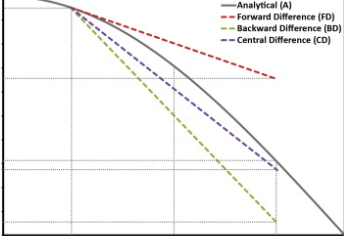
\includegraphics[width=0.45\textwidth]{figures/forward_vs_central_differentiation.png}
%       \caption{Comparison of Forward, Backward, \& Central Differentiation}
%       \label{forward_vs_central}
%       \end{center}
%       \end{figure}
%       \FloatBarrier
% 
% 
% 
% \paragraph{Method Specific Parameters:}
% 
% This section is specific to the method being used. In the above example it is specific to the $OPT++$ library. An additional example has been given below however if curious the reader is advised to see the default optimization methods located in:
% 
% \bigskip
% 
% \begin{lstlisting}
% $./data/cathode/optimization/optimization_methods_cathode/
% \end{lstlisting}
% or 
% \begin{lstlisting}
% $./data/mea/optimisation/optimization_methods_mea/
% \end{lstlisting}
% 
% \bigskip
% 
% In the following short example we are using a method from the SCOLIB library, the \texttt{coliny\_pattern\_search} algorithm. In this case we would change the \texttt{Optimization method = coliny\_pattern\_search} as appose to \texttt{optpp\_q\_newton} (\textit{line 17}).
% 
% We then would then replace (\textit{line 33 - 41}) in the above \texttt{opt\_app\_optimization} file  with the new method specific section.
% 
% \begin{lstlisting}
%      ######### Method Specific Parameters #########
%      #########              SCOLIB (COLINY)      #########
%      #########----------------------------#########
%       subsection coliny_pattern_search
%           set Initial Delta = 2                         # (default) 1
%           set Threshold Delta = 0.0001                        # (default) 0.0001
%       end
% \end{lstlisting}
% 
% 
% 
% \paragraph{Design Variables Section:}
% 
% The \texttt{Design Variables} Section is similar to the \texttt{opt\_app\_parametric} file except for two additional subsections.
% 
% \begin{enumerate}
%  \item 
% Scales
% 
% \item
% Step size
% \end{enumerate}
% 
% 
% \paragraph{Scales:} 
% 
% The scales section has two specifications 
% 
% \begin{enumerate}
%  \item 
% \texttt{scale\_method}
% 
% The \texttt{scale\_method} specifies whether you are going to specify no scale (\texttt{none}), \texttt{auto} scaling, \texttt{log}, or a \texttt{value}. In general it is good practice to specify a scale \texttt{value} as it allows the user to have a definite reference point, when using \texttt{auto} if there is a change in magnitude it will go unnoticed by the user in the final output solution. 
% 
% \item
% \texttt{scale} value
% 
% The scale value is the magnitude of the variable. For example if the variable is temperature we know that the scale is 100 as temperature is given in Kelvin (353 - 368 [K]). If its Nafion loading the scale is 0.1 as Nafion loading is a percentage (20 - 50 \%).
% \end{enumerate}
% 
% 
% 
% \paragraph{Step Size:}
% 
% The step size refers to the  $\bigtriangleup x $ in equations \ref{eq:Forward} \& \ref{eq:Central}. Greater the step size the less computations that will be required, however this also means the greatest error as the error is proportional to $(\bigtriangleup x)^2$. Therefore there is a fine trade off between computational time and error.
% 
% 
% 
% \paragraph{Responses Section:}
% 
% The Responses section has changes slightly compared to the \texttt{opt\_app\_parametric} file as we are now considering constrained optimization. If the above example was unconstrained optimization there would be no difference between the \texttt{opt\_app\_parametric} and \texttt{opt\_app\_optimization} responses section.
% 
% There are two types of constraints:
% 
% \begin{enumerate}
%  \item 
% Linear (Equality) Constraints (\textit{line 83})
% 
% \item
% Non-Linear Constraints (\textit{line 84})
% \end{enumerate}
% 
% In the above case we have three non-linear constrains and one linear constraint. 
% 
% 
% 
% \paragraph{Non-Linear Constraints:} 
% 
% Like the \texttt{Design Variable} section each nonlinear constraint requires a upper and lower bound (\textit{line 97 - 108}). If no finite upper or lower bound is to be specified $1e^{30}$ or $1e^{-30}$ can be specified.
% 
% 
% \paragraph{Linear (Equality) Constraints:} Unlike Non-Linear Constraints, Equality constraints only require the response variable to equal a value (\textit{line 112}). 
% 
% 
% 
% 
% 
% %-----------------------------------------------------------------------------------------------------
% %---------------------                                Running FCST
% %---------------------                        Multi-Objective Optimization
% %-----------------------------------------------------------------------------------------------------
% \section{Multi-Objective Optimization using OpenFCST} \label{sec:multi_objective_optimization}
% 
% To achieve multi-objective optimization we must first change three parameters.
% 
% \begin{enumerate}
%  \item 
% \texttt{Optimization strategy} (\textit{line 16})
% 
% \item
% \texttt{num\_design\_variables} (\textit{line 84})
% 
% \item
% \texttt{num\_objectives} (\textit{line 82})
% 
% \end{enumerate}
% 
% 
% 
% \paragraph{Optimization strategy}
% 
% When carrying out multi-objective optimization we can no longer optimize for just one objective function this is especially the case when an improvement of one objective comes at the expense of another (\textit{Performance \& Cost}). In order account for the additional objective function we incorporate weighting factors which specifies the importance of one objective over the other. The weights are referred to a \textbf{Pareto Weights} or \textbf{Pareto Set}.
% 
% In OpenFCST the default Pareto set is for two design variables. Figure \ref{pareto_set} below shows the  multi-objective weights for two design variables.
% 
% 
% 
% \FloatBarrier
% \begin{figure}[htbp]
% \begin{center}
% 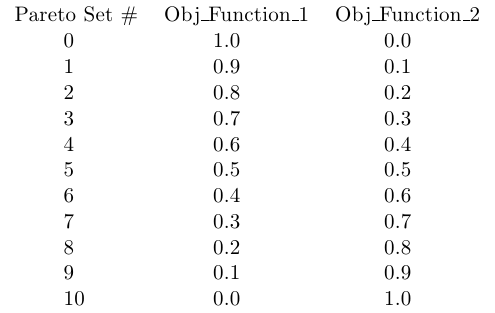
\includegraphics[width=0.4\textwidth]{figures/pareto_set.png}
% \caption{Pareto Set for 2 Design Variables}
% \label{pareto_set}
% \end{center}
% \end{figure}
% \FloatBarrier
% 
% 
% % \begin{center}
% %  
% % 
% % \begin{tabular}{lll}
% % Pareto Set \#       &Obj\_Function\_1 & Obj\_Function\_2 \\
% % 0   &        1.0    &        0.0    \\
% % 1   &        0.9    &        0.1    \\
% % 2   &        0.8    &        0.2    \\
% % 3   &        0.7    &        0.3    \\
% % 4   &        0.6    &        0.4    \\
% % 5   &        0.5    &        0.5    \\
% % 6   &        0.4    &        0.6    \\
% % 7   &        0.3    &        0.7    \\
% % 8   &        0.2    &        0.8    \\
% % 9   &        0.1    &        0.9    \\
% % 10  &        0.0    &        1.0    \\
% % \end{tabular} 
% % 
% % \end{center}
% 
% 
% 
% \paragraph{num\_design\_variables \& num\_objectives:}
% 
% Once the \texttt{Optimization strategy} has been set to \texttt{pareto\_set} we then change both the num\_design\_variables \& num\_objectives to 2 or whatever number of design variables are specified.
% At present OpenFCST like most multi-objective engineering problems, considers only two design variables however this can be easily modified by changing the default Pareto set found in \texttt{dakota\_application.cc}. 
% 
% \section{DAKOTA Methods} \label{dakota_methods}
% 
% The following list is all of the current DAKOTA Methods available as of \textbf{1-MAY-2013}. The methods are known to work with OpenFCST and can be utilized. For detailed discriptions on the individual methods see DAKOTA manuals.
% 
% \begin{multicols}{3}
% \begin{enumerate}
%     \item     \textbf{asynch\_pattern\_search}
%     \item       bayes\_calibration
%     \item       centered\_parameter\_study
%     \item       \textbf{coliny\_cobyla}
%     \item       \textbf{coliny\_direct}
%     \item       \textbf{coliny\_ea}
%     \item       \textbf{coliny\_pattern\_search}
%     \item       \textbf{coliny\_solis\_wets}
%     \item       \textbf{conmin\_frcg}
%     \item       \textbf{conmin\_mfd}
%     \item       dace
%     \item       dl\_solver
%     \item       dot
%     \item       dot\_bfgs
%     \item       dot\_frcg
%     \item       dot\_mmfd
%     \item       dot\_slp
%     \item       dot\_sqp
%     \item       \textbf{efficient\_global}
%     \item       fsu\_cvt
%     \item       fsu\_quasi\_mc
%     \item       global\_evidence
%     \item       global\_interval\_est
%     \item       global\_reliability
%     \item       importance\_sampling
%     \item       list\_parameter\_study
%     \item       local\_evidence
%     \item       local\_interval\_est
%     \item       local\_reliability
%     \item       \textbf{moga}
%     \item       \textbf{multidim\_parameter\_study}
%     \item       \textbf{ncsu\_direct}
%     \item       \textbf{nl2sol}
%     \item       nlpql\_sqp
%     \item       nlssol\_sqp
%     \item       nonlinear\_cg
%     \item       npsol\_sqp
%     \item       optpp\_cg
%     \item       \textbf{optpp\_fd\_newton}
%     \item       \textbf{optpp\_g\_newton}
%     \item       optpp\_newton                 % Needs the Hessian Matrix
%     \item       \textbf{optpp\_pds}
%     \item       \textbf{optpp\_q\_newton}
%     \item       polynomial\_chaos
%     \item       \textbf{psuade\_moat}
%     \item       richardson\_extrap
%     \item       sampling
%     \item       \textbf{soga}
%     \item       stanford
%     \item       stoch\_collocation
%     \item       surrogate\_based\_global
%     \item       surrogate\_based\_local
%     \item       vector\_parameter\_study
% \end{enumerate}
% \end{multicols}
% 
% 
% 
% 
% 
% 
% 
% %-----------------------------------------------------------------------------------------------------
% %---------------------                        Running OpenFCST
% %---------------------                        Optimization Path-line
% %-----------------------------------------------------------------------------------------------------
% \section{Fuel Cell Design \& Optimization Using OpenFCST}
% As we've seen above OpenFCST also has the capabilities to perform optimization studies. Any application that is inherited from \texttt{OptimizationBlockMatrixApplication} has the appropriate interface to be used for optimization studies. Information on how to run optimization can be found in sections \ref{Optimization_using_FCST} \& \ref{sec:multi_objective_optimization}.
% 
% To perform optimization studies, OpenFCST interfaces with the open source libraries DAKOTA developed by Sandia National Laboratory. For more information about the DAKOTA library please \href{http://dakota.sandia.gov/software.html}{click here}. The OpenFCST developers have developed an interface so that DAKOTA and OpenFCST can interact seamlessly. 
% 
% \subsection{OpenFCST classes that interact with DAKOTA (Developers Only)}
% Interaction between OpenFCST and DAKOTA is achieved by using \texttt{simulation\_builder} which will call the \texttt{run\_optimization()} function.
% 
% When OpenFCST is run as seen in figure \ref{analysis_schematic} the OpenFCST code is called on once in order to run a specific data point. However in parametric or optimization studies we require multiple points to be evaluated. This requires the use of the DAKOTA libraries in order to change the variables after each iteration. The two main files used to interface with DAKOTA are:
% 
% 
% \begin{enumerate}
%  \item 
% \texttt{dakota\_direct\_interface}
% 
% \item
% \texttt{dakota\_application}
% 
% \end{enumerate}
% 
% Once the initial stages of the code have been carried out by \texttt{simulator\_builder}, \texttt{simulator\_selector}, and \texttt{dakota\_application}, declaring and initialing all the variables from the \texttt{main\_app\_}, \texttt{data\_app\_}, \& \texttt{opt\_app\_} files. The \texttt{main.cc} file then proceeds to the \texttt{run()} function in \texttt{simulator\_builder.cc} (see below) in order to run the simulation.
% 
% In the \texttt{run()} function we can see in line 10 where the code checks to see if its running an analysis or parametric/optimization study, as explained in \ref{main_application_file}. During parametric/optimization studies the code will enter line 12 and proceed to the \texttt{run\_optimization()} function in \texttt{simulator\_builder.cc}. 
% 
% 
% \begin{lstlisting}
% template<int dim>
% void SimulatorBuilder<dim>::run()
% {
%       timer.restart();
%     
%       if (run_tests) run_test();
%       else
%       {
%               if (dakota_use || dakota_direct)
%               {
%                       run_optimization();
%               }
%               else
%               {
%                       //-- Select the application you want to run:
%                       app_lin = sim_selector->select_application();
%                       //-- Select the solver you want to run:
%                       newton = sim_selector->select_solver(app_lin.get());
%                       //-- Select the solving method you want to run, e.g. adaptive refinement:
%                       solver = sim_selector->select_solver_method(app_lin.get(), newton.get());
%                       // Here we have collected all information:
%                       deallog << "Run program using input file: " << simulator_parameter_file_name << std::endl;
%                       deallog.pop();
%                       solver->solve(simulator_parameter_file_name, param);
%                       timer.stop();
%               }
%       }
% 
%       timer.stop();
%       deallog.push("MAIN");
%       deallog << "The program was executed in: " << timer.wall_time() << " seconds " << std::endl;
%       deallog << "=============== END ====================" << std::endl;
%       deallog.pop();
%       
% }
% \end{lstlisting}
% 
% \bigskip
% 
% The main points to note once we enter the \texttt{run\_optimization()} function are:
% 
% \begin{enumerate}
% \item 
% Is DAKOTA running in Parallel or Series? (\textit{line 8})
% 
% As of \textbf{1-MAY-2013} Series is the only option available. This may change in the future.
% 
% \item
% Are we running a Non-Linear Least Squares (NLS) method or standard parametric/optimization routine? (\textit{line 16-25})
% 
% \end{enumerate}
% 
% \paragraph{Note:} 
% 
% These are questions that are answered in the \texttt{opt\_app\_} file explained earlier in section \ref{Optimization_using_FCST}.
% 
% 
% \bigskip
% 
% Once these have been specified the code will execute the \texttt{run()} function (\textit{line 28}), which begins the iterative loop until the parametric study has been complete or the stopping criteria have been met in optimization.An illistration of this can be see in figure \ref{dakota_optimization_interface} taken from Peter Dobson's 2012 paper.
% 
% 
% \begin{lstlisting}
% void SimulatorBuilder<dim>::run_optimization()
% {
%       deallog.pop();
%       if (dakota_direct)
%       {
%               // NOTE: Must declare these in order for parameter handler to not complain when reading the parameter file specified.
%               //        Not exclusively required for dakota application to run.
%               Dakota::ParallelLibrary parallel_lib;
%               shared_ptr<Dakota::ProblemDescDB> problem_db(new Dakota::ProblemDescDB (parallel_lib));
%               SIM::DakotaApplication optimization(problem_db, optimization_parameter_file_name);
%               optimization.declare_parameters(param);
%               optimization.manage_inputs(param);
% 
%               Dakota::DirectApplicInterface* optimization_interface;
%               
%               if (optimization.use_NLS())
%               {
%                       deallog<<"Entering DakotaLeastSquaresInterface"<<std::endl;
%                       optimization_interface = new SIM::DakotaLeastSquaresInterface<dim> (optimization, problem_db, param, sim_selector, simulator_parameter_file_name);
%               }
%               else
%               {
%                       deallog<<"Entering DakotaDirectInterface"<<std::endl;
%                       optimization_interface = new SIM::DakotaDirectInterface<dim > (optimization, problem_db, param, sim_selector, simulator_parameter_file_name);
%               }
%               
%               optimization.assign_interface(optimization_interface);
%               optimization.run();
%               
%               deallog << "Optimization completed" << std::endl;
% .
% .
% .
% \end{lstlisting}
% 
% 
% If running a standard parametric/optimization routine, the following \texttt{dakota\_direct\_interface} function will be used.
% 
% \begin{lstlisting}
% template <int dim>
% int DakotaDirectInterface<dim>::derived_map_ac(const Dakota::String& ac_name)
% \end{lstlisting}
% 
% If running a Non-Linear Least Squares (NLS) method, the following \texttt{dakota\_direct\_interface} function will be used.
% 
% \begin{lstlisting}
% template <int dim>
% int DakotaLeastSquaresInterface<dim>::derived_map_ac(const Dakota::String& ac_name)
% \end{lstlisting}
% 
% 
% \FloatBarrier
% \begin{figure}[htbp]
% \begin{center}
% 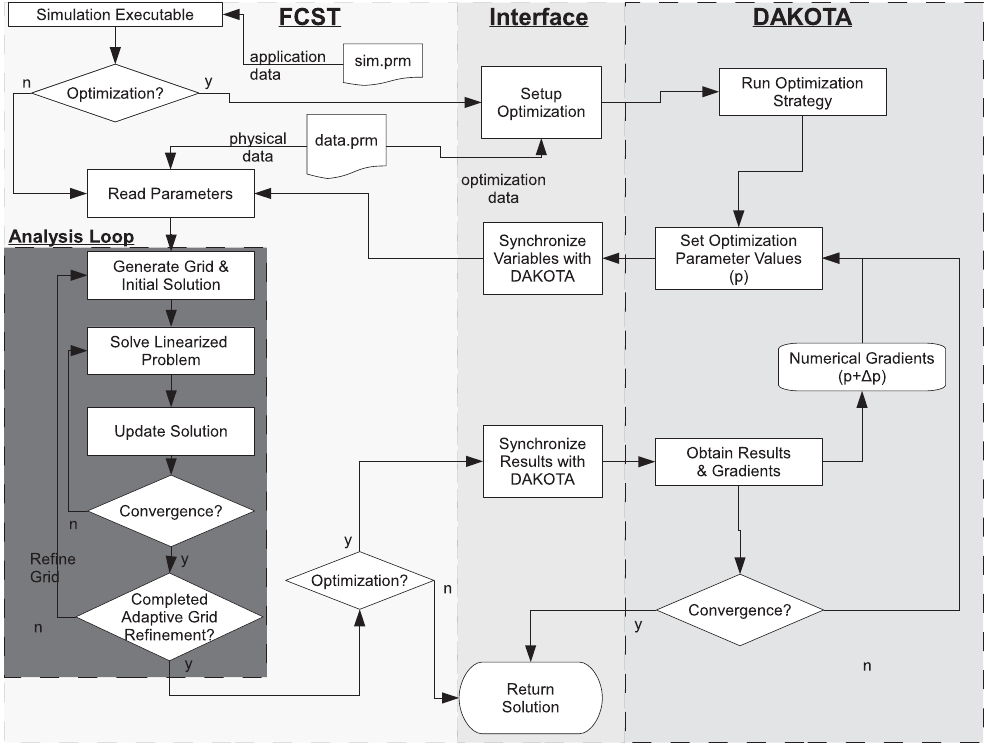
\includegraphics[width=1\textwidth]{figures/fcst_dakota_interface_Dobson.png}
% \caption{Schematic of Fuel Cell Analysis Code and DAKOTA Optimization Interface (Dobson, 2012)}
% \label{dakota_optimization_interface}
% \end{center}
% \end{figure}
% \FloatBarrier

%%===============================================================
%%===============================================================